\subsection{A quantitative approach}

\subsubsection{Agenda diversity}

% Agenda diversity

\par In order to quantify the similarities and differences between the Media Agenda and the Public Agenda, we start by asking how is the distribution of each agenda among the topic's space. In particular, we measure how diverse is each agenda. Following \cite{boydstun2014importance}, we calculate the normalized Shannon's entropy ($H$, see eq.\ref{eq:shannon_entropy}) in order to measure the diversity of the \textbf{MA} and \textbf{PA}.
\par In figure \ref{fig:shannon_entropy_agendas} we can see the value of $H$ as a function of time. We can see that there are periods where the diversity is lower than the usual. In particular, we pay attention to four dates in the Public Agenda which we detect as outliers of the typical behavior. The small value in the diversity is due to the fact that the most important topic attracts practically all the attention of the public, as can be seen in the radar plots included also in figure \ref{fig:shannon_entropy_agendas}. 
Two of the points belong to the topic \emph{Elections} and coincide with the primary and general legislative elections that took place in August 14th and October 22th. In the other hand, the other two point belong to the topic \emph{Missing person}: The first one a month after the disappearance of Santiago Maldonado, and the second one, when the Santiago Maldonado's body was found, a few days before the general legislative election (see section \ref{sec:Context}).

\begin{figure}[h]
\centering
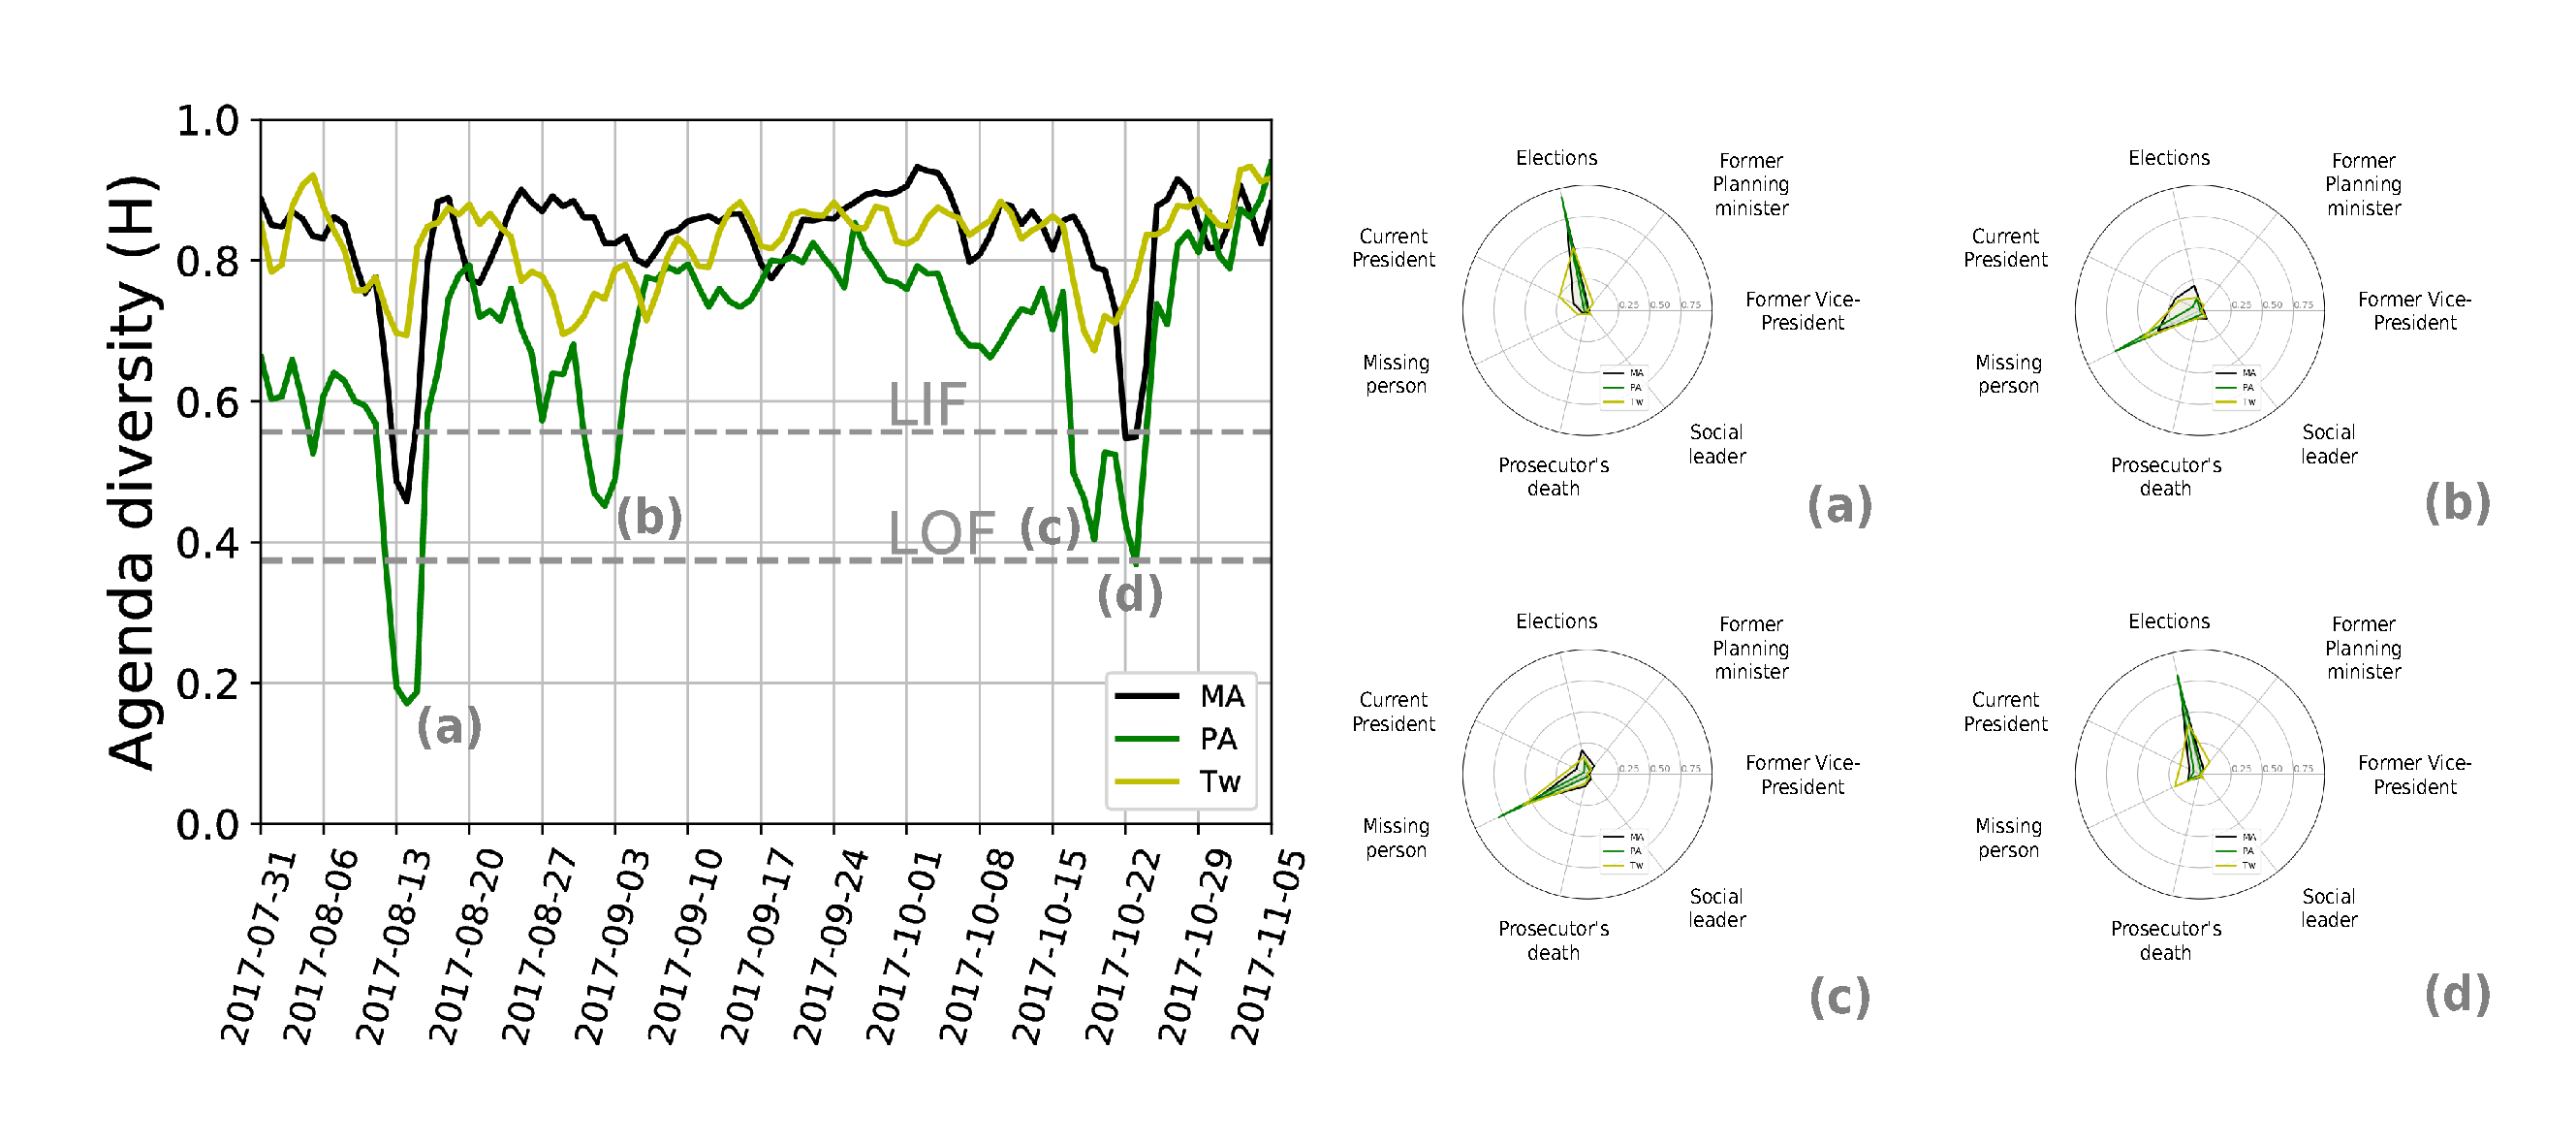
\includegraphics[width = \textwidth]{images/Fig3.pdf}
\caption{\textbf{Shannon entropy (H) as a measure of agenda diversity.} The Public Agenda show a less diverse behavior than the Media Agenda as can be seen in the left figure. The lower fences are shown in order to identify outliers. The related radar plots shows that those dates when the agenda has a low diversity, the most important topic catches the most public’s attention}
\label{fig:shannon_entropy_agendas}
\end{figure}

\par From the measure of $H$ we can also see that the median of the Public Agenda diversity ($H_{PA} = 0.70$) is lower than the each the Media Agenda's one ($H_{MA} = 0.85$) being this difference statistical significant ($p < 10^{-9}$).
We conclude that its an important fact about audience behavior: given a finite set of topics, \textbf{the Public Agenda is less diverse than the Media Agenda}, because the public seems to focus more in the most important topic than the Media can do.

\subsubsection{Public Agenda's distance}

% Jensen-Shannon distance between PA and MA

\par The measurement of the Shannon's entropy made above is an independent property of each distribution. 
Here we directly compare the Agendas by computing the Jensen-Shannon distance. We again identify outliers and aim to interpret them.
In figure \ref{fig:jensen_shannon_gt} we show the Jensen-Shannon distance as a function of time. We inspect three points that seems to be of particular interest. In all cases, the radar plots shows that a greater distance is associated with a more interest of public in the topic \emph{Missing person}. 
\par Points \textbf{(b)} and \textbf{(c)} shows that both the public and the Media are interest in that topic, but the Media have to cover other topics, so the distance value can be seen as a derivation of the diversity effect discussed in the last section.
However point \textbf{(a)} seems to show an interest of the public in the topic \emph{Missing person} that it is not reflected in the Media. In figure \ref{fig:all_agenda} we can see that this topic reached the first place in public's interest before that in the Media. We associate this fact with a campaign made in social media like Facebook and Twitter in August 26th, that paid for the appearance of Santiago Maldonado and had a great repercussion, maybe at first underestimated by the Media (see section \ref{sec:Context}). 
\par It is important to recall that it is our interpretation based on the knowledge of the context, and that we are not studying causality, i.e. we can't say, for instance, that in this case the Public Agenda set the Media Agenda. However, the Jensen-Shannon distance, in conjunction with the measurement of the agenda diversity given by the Shannon entropy, give an insight of independent behavior of the Public and the Media, and its identification can be a starting point to study the Media reaction to a change in audience's interests.
 
\begin{figure}[h]
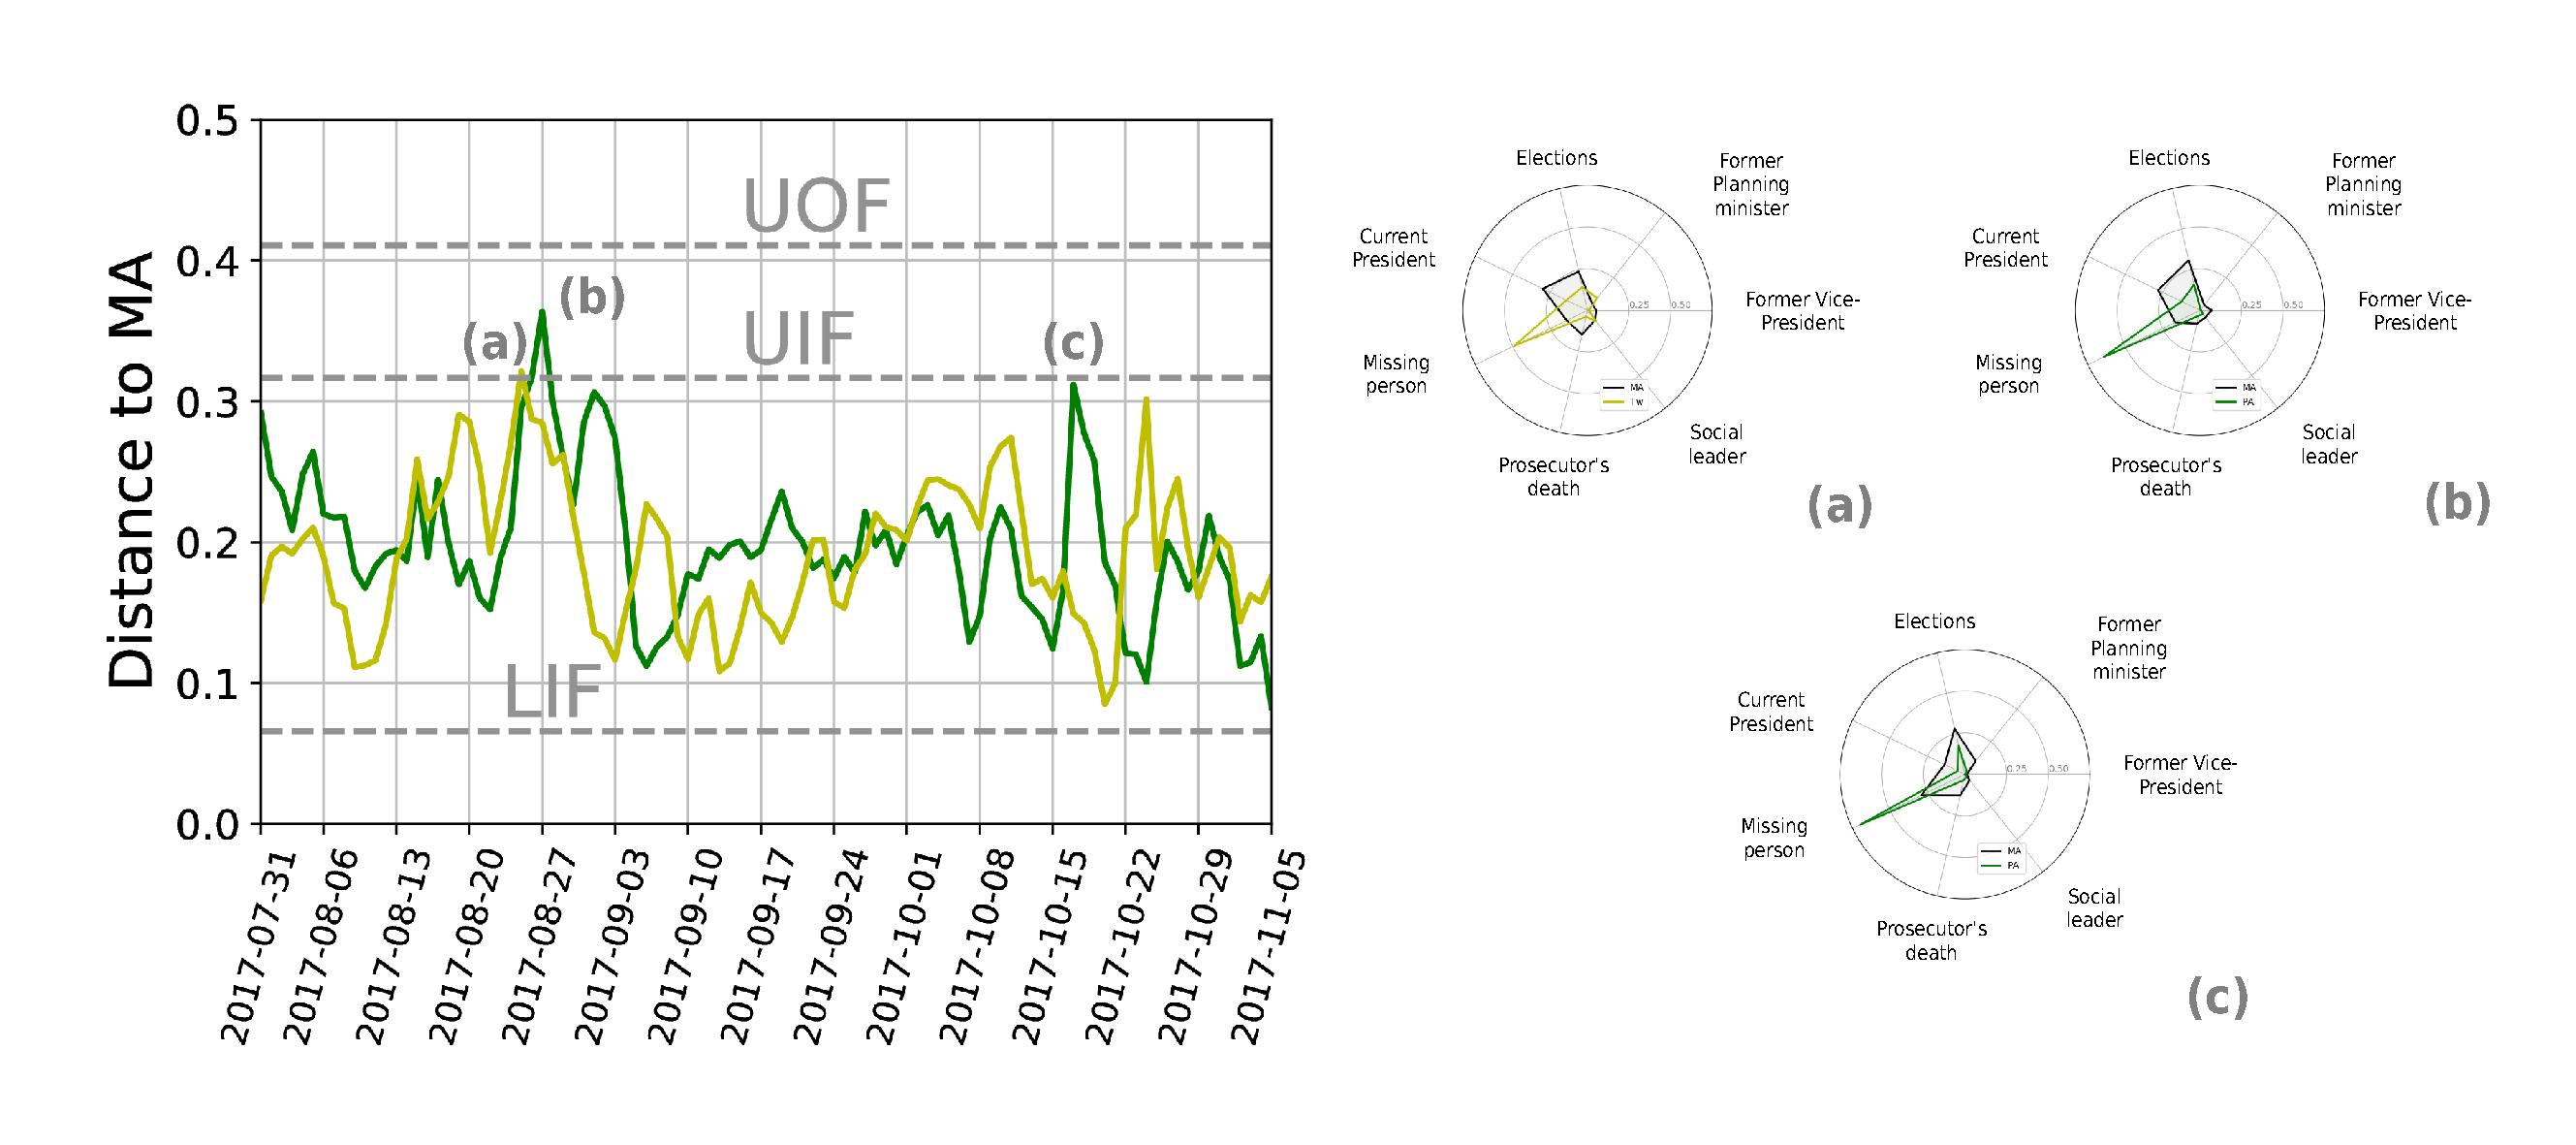
\includegraphics[width = \textwidth]{images/Fig4.pdf}
\caption{\textbf{Jensen Shannon distance between the Media Agenda and the Public Agenda as a function of time} (with the fences pointed out). The larger distances are due to a greater interest of the audience in the topic \emph{Missing person} which leads to lesser interest in the other topics, which the Media has to cover, maybe except in the date (a) where the Media seems not to anticipate the public interest in the mentioned topic.}
\label{fig:jensen_shannon_gt}
\end{figure}

